  
\section{The Z-Way software architecture}

Z-Way is a fully featured home automation controller supporting Z-Wave as communication technology. It allows to
\begin{itemize}
\item Include and exclude devices and configure these devices, manage the network configuration and stability by visualizing 
the configuration and routing within the network
\item Switch actuators such as electrical switches, dimmers, motor controls for sun blind, garage doors or venetian blind, door 
looks, heating thermostats and many more
\item Access sensor data such as motion detection, temperature, CO2, smoke etc.
\item Visualization of all functions of the Z-Wave network mapped to the floor plan or as tables simple to read
\item Create logical connection between events created by sensors and actions performed by actuators
\end{itemize}

Z-Way communicates (south bound) to the Z-Wave transceiver firmware (using the Serial Interface) and offers a 
northbound interface that complies to the JSON specification (for details about JSON see explanation in the chapters below).
This north bound Interface - referred to as JSON Interface - is used by applications or web pages (with Javascript)
 to operate and use the Z-Wave network. It is possible that multiple user interfaces or applications run in parallel and use the JSON 
 API. However in  case they send contradicting messages (one is turning off a device while one is turning on) the resulting
 state of the network is unpredictable. 

\begin{figure} 
\begin{center}
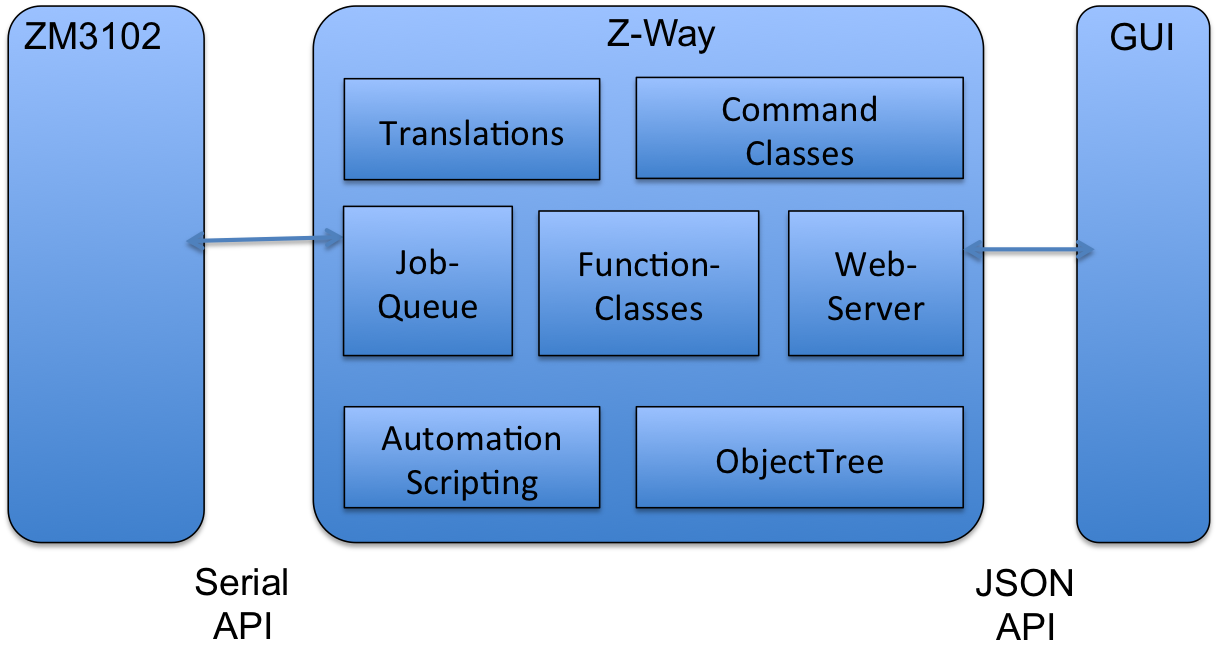
\includegraphics[scale=0.6]{pics/zway1en.png}
\caption{Z-Way Software Structure}
\label{zwaystructure} 
\end{center} 
\end{figure}

Z-Way consists of several function blocks:

\begin{itemize}
\item The Job Queue: This is the core of Z-Way
\item Function Classes: The implementation of all the commands to control the Z-Wave transceiver chip and the Z-Wave network
\item Command Classes: The application level commands used to control Z-Wave devices in the network
\item The JSON web server: It implements the application programmers interface
\item Translation Functions: They help to translate machine readable tokens into human-readable strings
\item The automation and scripting engine: This is the way to get the intelligence into the system.
\end{itemize}

 

\section{Z-Wave Basics}

\subsection{Network and controllers}

A Z-Wave network consists of various devices interconnected by a wireless communication protocol. Thanks to the Z-Wave standard 
{\bf products from different vendors can work together} seamlessly. 

Another advantage of Z-Wave is their ability to act as repeaters and forward data packets between nodes not able to communicate 
directly over the air. This extends the range of a Z-Wave network and improves stability. In order to perform this packet routing and 
forwarding the particular node needs to be mains powered. Battery operated nodes can not act as repeaters.

Z-Wave differentiates between portable and static controllers to control other devices. {\bf Portable controllers }change their location and 
they are battery powered. To allow long battery live time they are inactive most of the time and will only communicate with other 
devices during manual interaction (pressing a button). 

{\bf Static controllers} are installed on a fixed location. They are mains powered and therefore able to stay alive all the time to communicate 
with other devices. 

This allows static controllers to automatically update and optimize a Z-Wave network without further user interaction.  Z-Wave refers to 
his function as {\bf SUC/SIS (Static Update Controller/Static ID-Server) }as a special enhanced function of a static controller.

Beside the differentiation between static and portable controllers Z-Wave also distinguishes different roles of controllers in a network. 
The first controller of a network  - regardless if portable or static  - is always called {\bf primary controller}, while all further controllers – regardless 
if portable or static – are referred to as {\bf secondary controllers}.

In a standard network configuration the primary controller will organize the network and include and exclude other devices. Other controllers 
can be included but they will act as a secondary controller not being able to include further devices.

The special SUC/SIS function of a static controller enables all other controllers in a network to include further devices. Therefore the presence
 of such a SUC/SIS is highly desirable and Z-Way will always act in this enhanced mode if the Z-Wave hardware supports this  (Almost all current 
 USB Sticks support this mode).

If the hardware does not support the SUC/SIS mode the network will run in the standard mode (only the primary controller can include and exclude) 
 and Z-Way will try to turn on the SUC/SIS role at every other static controller which gets included.

Z-Way can be included as a secondary controller in other networks controlled by other Z-Wave controllers. Z-way will then follow the network 
 setup of this other network.

The “Network Management” tab of the demo user interface tells whether the software works in standard or in SUC/SIS mode.

\subsection{Inclusion and Configuration of various device types}

Z-Wave devices can be mains powered or battery operated.  The inclusion process for both devices types is similar, however battery operated devices need special handling.

\subsubsection{Mains Powered Devices}

A Mains powered device is easy to configure after inclusion since the device will receive all configuration commands and execute them immediately. 
 Mains powered devices are always listening to other commands and can repeat commands to other nodes. 

\subsubsection{Battery Operated Devices}

The main objective of a battery-operated device is to preserve the battery power and only use as much battery power as needed.  Battery powered devices 
 are therefore in a deep-sleep state most of the time. In deep-sleep state they are not able to communicate with other devices. 

In order to communicate with other device the battery-operated device needs to be woken up and send to sleep mode right after the communication 
 took place. To maintain a minimal level of “responsiveness” and to allow to configure and to use battery-operated devices Z-Wave offers three basic solutions:
\begin{itemize}
\item	Devices with wakeup intervals
\item Frequently listening battery devices 
\item Devices with manual wakeup
\end{itemize}

\begin{quote}

{\bf Wakeup Interval}
\end{quote}
Devices with wakeup interval will wakeup after a defined interval and send out a wakeup notification. Other devices such as the Z-Way controller are 
able to communicate with this device and send out messages to this device (The controller know about the status of the battery operated device and will 
queue messages in a waiting queue.) After all communication is done the controller is supposed to send the device back into deep sleep.
If no communication happens the battery-operated device will go back into deep sleep mode after a defined time (typically some seconds – up to one minute).

The best practice of Z-Wave suggests that battery operated devices stay awake for a defined time right after inclusion and go into deep sleep mode 
afterwards. This first awake-time is device dependent and varies from 1 minute to one hour.

Hence it is recommended to configure the device right after inclusion to make sure the device is still alive. If the battery operated device is already in 
sleep state all configuration commands will be queued and executed after the next scheduled wakeup if and only if a valid wakeup interval was configured 
during the first part of the configuration process. If this was not the case the device needs to be woken up manually.

If the device went already into deep sleep before the configuration was finished it is recommended to wake up the device manually to speed up the c
onfiguration process. Otherwise the configuration will happen after the next scheduled wakeup.

Some battery-operated devices may not go into sleep mode at all after inclusion but need to be sent into deep sleep after configuration is finished. 
This is done by Z-Way automatically.

The configuration of the wakeup interval is a tradeoff between maximum battery life-time  (suggest a very long wakeup interval with few wakeup cycles) 
and some responsiveness of the device in case of a network-reorganization. Typical values are 5 min … 5 hours.

\begin{quote}
{\bf Frequently Listening Devices}
\end{quote}
Z-Wave has introduced frequently listening devices (FLIRS). These devices will wakeup at least once in a second and try to receive a message. The trick 
is that the wakeup is so short, that on average the power consumption of FLIRS devices are low enough to allow battery life times greater than one year. 
FLIRS devices can be configured without any problems like mains powered devices since every command will always be received latest after one second.
However FLIRS device will not route other devices messages to preserve battery power.
\begin{quote}
{\bf Devices with manual wakeup}
\end{quote}
Remote controls are battery operated as well but they are only awake if a button is pressed. Remote controls will not wakeup regularly to check for queued 
messages. Hence whenever a remote control is configured from the Z-Way controller, the device needs to be woken up manually. Please refer to the manual 
of the remote control for further instructions how to wakeup the device.  

\subsection {Network Stability}

Wireless communication is a challenging task. Therefore Z-Wave has implemented quite a few approaches how to make communication over the air more reliable.

The most important of these approaches is the so called meshing, which means that every mains powered node is able to store and forward packets on behalf
 of other nodes in case there is no direct wireless communication between transmitter and receiver.

To allow meshing in a network the controller needs to know a map of all available links between nodes. A link between nodes is referred to as stable wireless 
 communication between these two links. Knowing all these links the controller can calculate routes (ways) to communicate to devices and inform other devices 
 accordingly (an association set will cause two nodes to communicate with each other without using the controller). 
The routing within a Z-Wave network is based on fixed predefined routes. Each packet, which is supposed to be sent using other nodes, has the full information 
 about the desired route in the packet header. It is not possible to change this route on the fly.

While this sounds quite inflexible this is in fact quite smart. It significantly reduces traffic over the air and attempts to follow wrong routes.  

If the attempt to communicate with a certain device over a given route fails (no acknowledge received back) the controller will try two more times the same route 
 and then a number of other possible route to reach the device. This is also very smart because the route may be intercepted by a failed or otherwise not available 
 node but the final destination is still alive and working well.

If the communication attempt fails the controller will try again and again to communicate with the desired target always creating a lot of traffic 
by testing other available routes.  This behavior is still desired but the increased traffic may slow down other communication in the network and will particularly keep the 
 controller chip busy. A result of this traffic is the delayed executions of other wireless commands such as turning on a light.

The controller will stop to try communicating to this device at a certain time, which depends on the size and complexity of the network. The controller will mark 
 the device as failed and ignore any further communication request to this link unless receiving an unsolicited message from this disappeared device.

The worst-case scenario is that the device is only reachable occasionally since this will always motivate the controller to try as hard as he can 
to reach the  device. That again causes a lot of traffic and delay for other command executions.

There are a couple of best practices to minimize these traffic overhead and keep the network in a stable status with minimal wireless traffic and minimal response
  time to wireless commands sent.
\begin{enumerate}
\item Exclude devices which are not longer needed or which are moved outside the network. If you take one device  - e.g. a wall plug- and bring him outside the 
  network, you need to exclude him from the network. Otherwise this device is not reached anymore and will create overhead traffic until it’s marked as failed.
\item If a device is obviously failed or broken, remove it using the “Remove Failed Node” function in the “Network Management” tab.
\item If a device is moved within the network you need to start network reorganization. This process asks each node to detect its neighbors 
and reports the list of neighbors back to the controller. This is used to update the routing table and recalculates the best routes to the devices.
\item Try to avoid longer routes. Check the routes between two nodes using the “routing table” tab and refer to the advice giving in the manual chapter “Routing Table”.
\item Avoid “shaky” links. The tab “Communication Timing” in the expert’s mode in tab “Routing table” gives valuable information about the quality of wireless links. 
\item Reduce Polling intensity. On default a script “ Polling devices” in the network zone will be called every minute and poll a list of command class if they are available on the device. This will create increasing overhead if the network grows.  Make sure only to poll what it absolutely needed.
 \begin{itemize}
\item You may want to increase polling interval from one minute to 5 minutes or so.
\item Don not poll FLIRS devices and don not try to poll devices that are marked as “failed”.
\item Try to enable pushing of sensor values wherever possible. Most metering devices (power, temperature) allow to be configured so that they 
send sensor updates frequently or when changes occur. Make heavy use of these functions and limit the polling of the corresponding command classes
\item Meter command classes reporting accumulated values do not need to be polled so often.
\item If there is already one devices class polled delivering the status of a device – e.g. switch binary command classes for a binary switch – there is no need to poll additional command classes  - e.g. the basic command class- to get the very same value. 
 \end{itemize} 
\end{enumerate}
Network reorganization is also a good prevention practice and it is recommended after any change of the network (include device, exclude devices remove 
 failed nodes, move nodes,) it takes a couple of minutes and updates the routing table. Please be aware that changes in the environment such as new furniture
may also change the wireless communication environment. A regular network reorganization is therefore a good practice to keep the network healthy and stable.
